\documentclass[12pt]{article}
\usepackage[margin=1.0in]{geometry}
\usepackage[utf8]{inputenc}
\usepackage[T1]{fontenc}
\usepackage{lmodern}
\usepackage[spanish]{babel}
\usepackage{amsmath}
\usepackage{graphicx}
\usepackage{multicol}

\title{Clase 3}
\begin{document}
\maketitle


\begin{equation}
\int\limits_{x}^{j}
\end{equation}

\begin{figure}
\centering
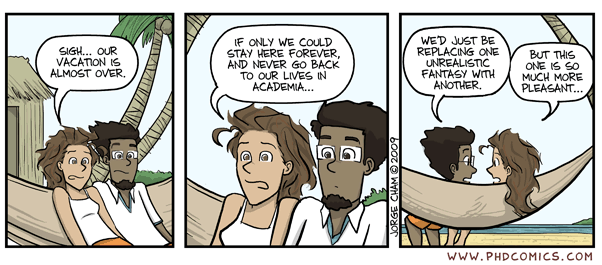
\includegraphics[scale=0.6]{f1.png}
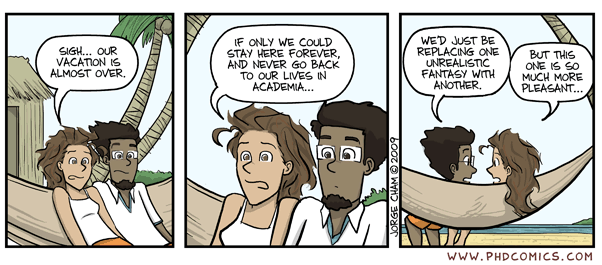
\includegraphics[scale=0.6]{f1.png}
\caption{Mis Vacaciones \label{fig:vacaciones}}
\end{figure}

Entonces en la Fig.\ref{fig:vacaciones} se muestran mis vacaciones.


\section{Tablas}

\begin{table}
\begin{center}
\begin{tabular}{c c c}
\hline
\hline
Distancia & Edad & Tiempo\\
\hline
10 & 20 & 30 \\
$\dfrac{x}{y}$ & 50 & 60\\
\hline 
\end{tabular}
\end{center}
\caption{Propiedades \label{tab:prop}}
\end{table}


Entonces en el Cuadro \ref{tab:prop} se muestran...


\begin{multicols}{2}
"The album is produced once again by Loris Ceroni (who produced before artists like Fey, Natalia Lafourcade and Laura Pausini. 13 tracks were selected including songs written by José Luis Pagán, Mario Domm and the singer herself. The album was released in Mexico and Latinamerica and later in the United States" \cite{Lafourcade}

\end{multicols}


\begin{verbatim}
fd iqdf-\*~~~"_ \item
\end{verbatim}

\begin{thebibliography}{1}
\bibitem[Lafourcade et.al]{Lafourcade}https://en.wikipedia.org/wiki/Fuerza
\end{thebibliography}
































































\end{document}














